\documentclass[aspectratio=169]{beamer}

\usetheme[secheader]{Boadilla}
\usecolortheme{crane}
\usepackage[latin1]{inputenc}

\title{Open Source Android Development Tools}
\author{Manfred Moser}
\date{June, 2011}
\institute[2011]{simpligility technologies inc.\\[\medskipamount]
      
\includegraphics[scale=0.6]{simpligility.png}%
 }

\logo{
\includegraphics[scale=0.25]{simpligility.png}}
\newcommand{\surl}[1] {{\tiny \url{#1}}}

\begin{document}

\begin{frame}
  \titlepage
\end{frame}

\begin{frame}{Table of Contents}
  SDK, ADT and beyond
  \setcounter{tocdepth}{1}
  \tableofcontents
\end{frame}

%\begin{frame}{About Manfred}

%\end{frame}


\section{Android Itself}

  \subsection{Components}
    \begin{frame}{What components make up Android codebase?}
      \begin{description}
        \item<1->Android Proper - as found on your device
        \item<2->Android Open Source Project AOSP - subset of above 
        \item<3->Android Software Development Kit SDK - for Java based development applications
        \item<4->Android Native Development Kit - for C/C++ based development
        \item<5->Android Open Accessory Development Kit ADK - for USB based hardware hacking
        \item<6->Android Development Toolkit ADT - Eclipse plugin for Android development  
    \end{description}
    \end{frame}

  \subsection{Android Proper}
    \begin{frame}{Android Proper - As Found on Your Device}
    \begin{description}
      \item<1->Linux
      \item<2->Apache Harmony 
      \item<3->Lots of other open source components
      \item<4->AOSP bits
      \item<5->binary device driver and other blobs 
      \item<6->custom parts from manufacturer and provider
    \end{description}
    \end{frame}
  
  \subsection{AOSP}
    \begin{frame}{Android Open Source Project AOSP}
      \begin{description}
        \item<1->open source drops
        \item<2->base for custom roms and such
        \item<3->numerous specific components e.g. Dalvik
        \item<4->various forks from upstream projects
      \end{description}
    \end{frame}

  \subsection{ADT}
    \begin{frame}{Android Development Toolkit ADT}
      \begin{description}
        \item<1->open source, fully 
        \item<2->EPL
      \end{description}
    \end{frame}

\section{Development Tools}

  \subsection{IDEs}

    \begin{frame}{Eclipse and ADT and friends}
      
    \end{frame}

    \begin{frame}{Other IDE's}
      \begin{description}
       \item<1->[Motorola Motodev Studio for Android] \hfill \\  partly open source, commiting upstream to ADT and Eclipse Sequabout motodev, some bla bal
\item<2->[Jetbrains IntelliJ IDEA CE] \hfill \\ fully open source, includes Android support
        \item<3->[Oracle Netbeans] \hfill \\ fully open source, community plugin for Android
\surl{http://kenai.com/projects/nbandroid/}
\end{description}

    \end{frame}


  \subsection{Build Tools}

    \begin{frame}{Maven Android Plugin and Friends}
      \begin{description}
       \item Maven Android Plugin \surl{http://code.google.com/p/maven-android-plugin/}
       \item Maven Android SDK Deployer \surl{https://github.com/mosabua/maven-android-sdk-deployer}
       \item Android4Maven \surl{http://sourceforge.net/projects/android4maven/}
       \item M2E Android \surl{https://github.com/rgladwell/m2e-android}
       \item AndroidSDKFido \surl{https://github.com/joakime/android-sdkfido}
       \item Android RIndirect \surl{https://github.com/akquinet/android-rindirect}
      \end{description}

    \end{frame}

    \begin{frame}{Others}
      \begin{description}
       \item Gradle Android Plugin \surl{https://github.com/jvoegele/gradle-android-plugin}
       \item SBT Android Plugin \surl{https://github.com/jberkel/android-plugin}
      \end{description}
    \end{frame}

    \begin{frame}{Maven Android Plugin - Example}
      \begin{itemize}
       \item deploy to multiple devices
       \item reuse of Maven plugins
       \item use of libraries and Android components easy
      \end{itemize}
    \end{frame}

  \subsection{Other Languages}
    \begin{frame}{Other Languages}
      Java is main language for development and API but also possible are 
      \begin{itemize}
      \item C/C++ (via NDK first class)
      \item JRuby
      \item Scala
      \item C\#
      \item JavaScript
      \item Processing \surl{http://wiki.processing.org/w/Android}
      \end{itemize}
    \end{frame}

    \begin{frame}{Example - Scala libraries}
      \begin{itemize}
       \item Baitha \surl{https://github.com/sattvik/baitha}
       \item Positronic Net \surl{https://github.com/rst/positronic_net}
      \end{itemize}

    \end{frame}



  \subsection{Other Development Tools}

    \begin{frame}{Other Development Tools}
      \begin{description}
      
        \item<1->Droid at Screen \surl{http://blog.ribomation.com/2010/01/droidscreen/}
        \item DroidDraw \surl{http://www.droiddraw.org/} 
        \item<2->dex2jar \surl{http://code.google.com/p/dex2jar/}
        \item[smali/baksmali] \hfill \\ dex assembler/disassembler \surl{http://code.google.com/p/smali/}
        \item<3->Android2PO - Converter Android strings to gettext \surl{https://github.com/miracle2k/android2po}
      \end{description}
   \end{frame}

\section{Development Libraries}


  \subsection{Java Libraries}

    \begin{frame}{Java Libraries suitable for Android}
      \begin{itemize}
        \item<1->jackson
        \item<2->gson
        \item SimpleXML \surl{http://simple.sourceforge.net/home.php}
      \end{itemize}
    \end{frame}

  \subsection{Android Specific Libraries}

    \begin{frame}{Android Specific Libraries}
      \begin{itemize}
        \item<1->Roboguice \surl{http://roboguice.org} 
        \item<2->AndroidAnnotations \surl{http://code.google.com/p/androidannotations/}
        \item<3->DroidFu \surl{http://github.com/kaeppler/droid-fu}
        \item<4->OpenIntents \surl{http://code.google.com/p/openintents/}
        \item<5->AndEngine \surl{http://www.andengine.org/}
        \item<6->ksoap2-android \surl{http://code.google.com/p/ksoap2-android/}
        \item<7->WSDL2Android \surl{https://github.com/kigero/WSDL2Android}
        \item<8->CommonsWare Android Components CWAC \surl{https://github.com/commonsguy}  
        \item<9->AndroidAsync \surl{https://bitbucket.org/hal/android-async/}  
        \item DroidKit\surl{https://github.com/droidkit/droidkit}
\end{itemize}
    \end{frame}

    \begin{frame}{Example RoboGuice}
      logo, code sample
    \end{frame}
  

  \subsection{Android UI Libraries}

    \begin{frame}{UI Libraries}
      \begin{itemize}
       \item<1-> GreenDroid \surl{https://github.com/cyrilmottier/GreenDroid}
       \item<2-> ActionBarSherlock \surl{http://actionbarsherlock.com/} 
       \item Android Wheel \surl{http://code.google.com/p/android-wheel/}
      \end{itemize}

    \end{frame}

    \begin{frame}{AndroidSherlock}
      \begin{center}
      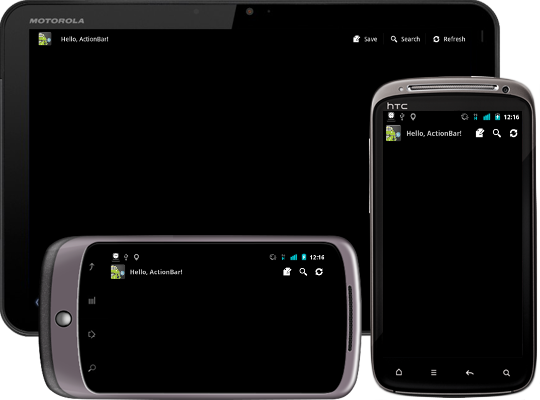
\includegraphics[height=1.0in]{androidsherlock.png}
      \end{center}
    \end{frame}

  \subsection{Android Testing Libraries}

    \begin{frame}{Android Testing Libraries}
      \begin{itemize}
        \item<1->Robotium \surl{http://robotium.org}
        \item<2->Robolectric \surl{http://robolectric.org}
        \item<3->Calculon \surl{https://github.com/kaeppler/calculon}
        \item<4->Android JUnit Report \surl{https://github.com/jsankey/android-junit-report}
      \end{itemize}
    \end{frame}

    \begin{frame}{Testing Demo}
      \begin{itemize}
       \item Robotium
        \item Robolectric
      \end{itemize}

    \end{frame}



  \subsection{Others of interest}  

    \begin{frame}{i-jetty}
      \begin{itemize}
       \item i-jetty \surl{http://code.google.com/p/i-jetty/}
      \end{itemize}

    \end{frame}

    \begin{frame}{web based frameworks}
    \end{frame}

\section{Conclusions}

  \subsection{Android = Java?}
    \begin{frame}{Is Android Java?}
      \begin{itemize}
      \item<1-> Yes - default application programming language
      \item<2-> Yes - API is Java based
      \item<3-> No - not using a standard compliant Java Virtual Machine Runtime
      \item<4-> No - only using parts of the standard class libraries and 
      \end{itemize}
    \end{frame}

  \subsection{Android = Open Source?}
    \begin{frame}{Is Android Open Source?}
      \begin{itemize}
       \item<1-> Yes, in time - AOSP open sourced in drops
       \item<2-> Yes -ADT fully open source
       \item<3-> Yes and no - cooperation with upstream projects patchy but exists
       \item<4-> No - binary blobs for drivers and other parts
      \end{itemize}
    \end{frame}

  \subsection{Android part of Java Community?}
    \begin{frame}{Android part of the Java Community?}
     \begin{itemize}
      \item<1-> Yes - parts of Android itself
      \item<2-> Yes - tooling around Android
      \item<3-> Yes - lots of libraries and tooling from rest of Java universe
      \item<4-> Yes - lots of people from Java community, also part of Android community
      \item<5-> Yes - lots of JVM related aspects as well e.g. Scala, JRuby, Processing, Groovy...
      \end{itemize}
    \end{frame}
  
  \subsection{Android part of Open Source Community?}
    \begin{frame}{Android part of Open Source Community?}
     \begin{itemize}
      \item<1-> Yes - part of Apache Community
      \item<2-> Yes - part of Eclipse Community
      \item<3-> Yes - part of Ruby, Scala, Groovy/Gradle...
      \item<4-> Yes - lots of open source libraries specifically to Android
      \item<5-> Yes - lots of projects on Github, Google Code, ...
      \item<6-> Yes - move towards Maker community with ADK
     \end{itemize}
    \end{frame}

  \subsection{Overall Conclusions}
    \begin{frame}{Overall conclusion}
      \begin{itemize}
        \item<1-> Despite lots of flaws and kinks, makes it interesting ;-)
        \item<2-> Android is part of the Java and Open Source communities
        \item<3-> Android touches a lot more communities and brings them together
        \item<4-> Android is a great chance to unify and collaborate 
      \end{itemize}
    \end{frame}

  \subsection{What can you do?}
    \begin{frame}{What can you do?}
      \begin{itemize}
        \item<1-> Buy an unlocked/unlockable device
        \item<2-> Use a custom ROM
        \item<3-> Ask for open source drops of AOSP 
        \item<4-> Encourage patches to upstream projects and 
        \item<5-> Ask for open sourcing of any closed parts, tools...
        \item<6-> Contribute and cooperate yourself! 
      \end{itemize}
    \end{frame}
\end{document}